%!TEX root=../../../main.tex

Using the base annotation model as a starting point, the targeted document
commenting feature can be implemented. In this scenario, the \textit{``where''}
field of the base model needs to encode both the document identifier and the
exact target of the annotation (e.g., the second page).

In the current version of Invenio, records can have one or more documents
associated, each of them with multiple versions. For example, during the CDS
paper review rounds, a single record will be used to upload multiple drafts of
the same document. Thus, annotations need to be attached to the correct version
of documents, in order to avoid displaying obsolete information. As the document
storage model is currently changing for the next version of Invenio, we have
chosen to implicitly attach annotations to the latest version of record
documents; nevertheless, this can be changed with minimal effort due to the
customisable nature of the JSON models.

Regarding the document locations to which annotations can refer, after studying
over one thousand comments from CDS review rounds, we have chosen a total of
nine so-called \textit{``marker''} which can identify valid targets:
\begin{enumerate}
  \item Page (P)
  \item Figure (F)
  \item Line (L): this refers to the text line number which is sometimes used
                  in drafts (e.e., LaTeX documents allow this when using the
                  \textit{``draft''} option for the document class. Optionally,
                  this could also be used in other configurations as, for
                  example, specifying a row in a table or a relative line in a
                  paragraph.
  \item Equation (E)
  \item Table (T)
  \item Section (S): this could also refer to subsections as long as they
                     possess a proper identifier (e.g., Subsection 4.2).
  \item Paragraph (PP): this will likely refer to relative positions, such
                        as \textit{``the third paragraph on the third page''}.
  \item Reference (R): a bibliographic citation, could prove useful in a
                       scenario similar to the INSPIRE reference correction 
                       form presented in Section \ref{sec:motiv}.
  \item General (G): this allows specifying annotations which regard general
                     aspects, such as formatting issues (\textit{``the text is
                     not justified''}.
\end{enumerate}
The letters between parentheses above denote the special markup that can be used
by users for referring to the various document locations; for example,
\textit{``P.2: F.3a: equation system is not presumed''} is a valid annotation
on subfigure $3a$ on the second page. As can be seen, markers can be combined to
form hierarchic structures with no depth restrictions; this should help in
specifying precise, unambiguous locations.

This type of annotations can be inserted by using the standard Invenio
commenting facilities in two different manners:

\begin{itemize}
  \item Online, by using the form in Fig. \ref{fig:commentform}, which also
        provides a brief usage tutorial. Moreover, the aggregated view window in
        Fig. \ref{fig:noteview} can be used to point-and-click on the document
        previewer pane to add an annotation on the currently previewed page (the
        input form is pre-filled with the necessary markup).
  \item Offline, by using the described markup to edit the annotations while
        online access to the Invenio instance is not possible. Users can write
        their review, decorate it with the markup and add it later through the
        online form described above in order to be included with the rest of the
        comments. This is the reason for the markup being visible to the users
        and not implicit, directly encoded in the system by means of, for
        example, an interface similar to the one in Fig. \ref{fix:noteview}.
\end{itemize}

FIXME: fig:commentform

All the added record comments will be scanned and valid annotations will be
extracted by means of a simple regular expression mechanism. From a high level,
annotations are considered valid if complying with the following format:
\begin{verbatim}
  <MARKER 1>: [<MARKER 2>: ... [<MARKER N>:]] <FREE TEXT>
\end{verbatim}
Each annotation is expected to be preceded and followed by at least one new
line character.

Extracted annotations will be saved in a JSON document complying with the
JSONAlchemy template, in the MongoDB database. To summarise, the model for
targeted document annotations is similar to the base one presented in Section
\ref{sec:gra}, except for the \textit{``where''} field which includes the
record identifier and document marker(s), and a new field containing the
identifier of the comment in which the annotation originated (used for
providing context to end-users). The workflow of document annotations is
pictured in Fig. \ref{fig:docanno}.

\begin{figure}[!ht]
  \centering
  \fbox{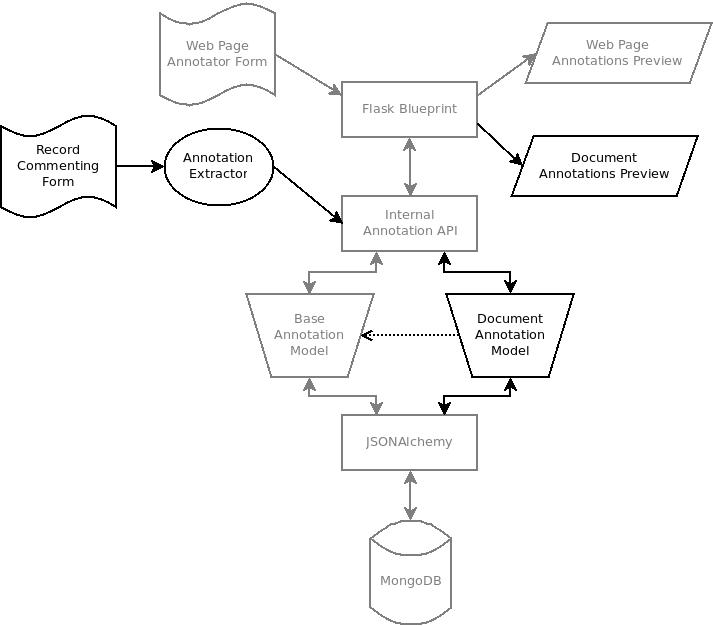
\includegraphics[scale=0.6]{static/dia/doc_anno.jpeg}}
  \caption[Document annotation workflow]
          {Document annotation workflow; the base annotation model is extended
           to allow adding notes on specific document locations (e.g., page
           figure, equation). Annotations are extracted from basic Invenio
           comments, by identifying the special markup that can be employed by
           users to refer to locations.}
  \label{fig:docanno}
\end{figure}

Finally, annotations can be previewed in a manner similar to the one presented
in Fig. \ref{fig:noteview}. The current version proposes a two-column window,
with one column dedicated to previewing the concerned document (currently the
supported format is PDF), and the other to displaying the annotations. Coming
back to the CDS review process use-case, the annotation display has been
designed in order to address two issues:
\begin{enumerate}
  \item Separate items from free-text comments: even if a comment includes both
        punctual remarks and also non-structured content, the aggregated view
        will display only the notes targeting a specifying aspect. Considering the
        following comment:
        \begin{verbatim}
          Dear authors,

          This is a very good paper, but I have the following remark:
          P.2: F.3a: equation system is not presumed 

          Regards,
        \end{verbatim}
        only the remark on subfigure $3a$ on the second page will be displayed.
  \item Aggregate remarks by location, to allow the authors in charge of
        amending the paper to systematically follow them. As can be observed in
        Fig. \ref{fic:noteview}, annotations are first grouped by page and then
        hierarchically, in a top-down manner, from the most general marker to
        the most particular one.
\end{enumerate}

FIXME: fig:noteview
